% 2010 Zhejiang science Q19: ball-pipe network. Top inlet M, bifurcating double-wall
% pipes (schematic wall tracing), three outlets C (left), A (middle), B (right).
% Solid walls only, no arrows; filled dot at M.
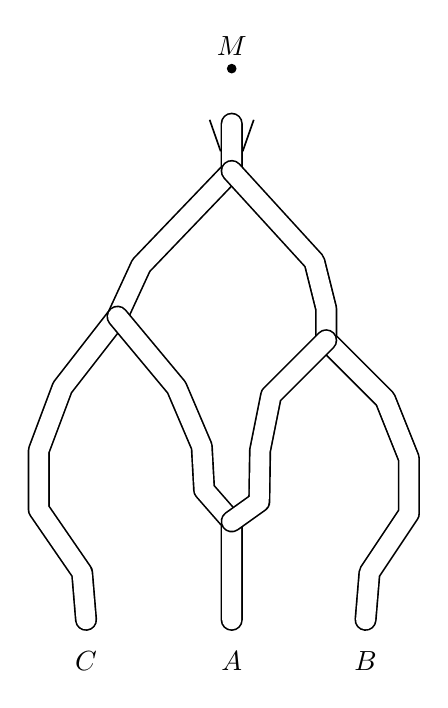
\begin{tikzpicture}[line width=.6pt, font=\normalsize]
\tikzset{d/.style={circle, fill, inner sep=0pt, minimum size=3.5pt}}
\node[d] (M) at (0,7) {}; \node[above=1pt] at (M) {$M$};
% pipe centre-line skeleton, drawn as double walls (pipe interior stays white);
% each run is one continuous path so walls stay smooth, runs meet at forks
\tikzset{pipe/.style={double, double distance=2.4mm, line join=round, line cap=round}}
% left run: outlet C up to inlet
\draw[pipe] (-1.85,0) -- (-1.9,0.6) -- (-2.45,1.4) -- (-2.45,2.15)
  -- (-2.15,2.95) -- (-1.45,3.85) -- (-1.15,4.5) -- (0,5.7) -- (0,6.3);
% middle-left run: outlet A up to left fork
\draw[pipe] (0,0) -- (0,1.25) -- (-0.35,1.65) -- (-0.38,2.2)
  -- (-0.7,2.95) -- (-1.45,3.85);
% right run: outlet B up to inlet
\draw[pipe] (1.7,0) -- (1.75,0.6) -- (2.25,1.35) -- (2.25,2.05)
  -- (1.95,2.8) -- (1.2,3.55) -- (1.2,3.95) -- (1.05,4.55) -- (0,5.7);
% middle-right run: centre junction up to right fork
\draw[pipe] (0,1.25) -- (0.35,1.5) -- (0.36,2.15) -- (0.5,2.85) -- (1.2,3.55);
% short inlet lips below M
\draw[line width=.6pt] (-0.28,6.35) -- (-0.14,5.95);
\draw[line width=.6pt] (0.28,6.35) -- (0.14,5.95);
\node[below=8pt] at (-1.85,0) {$C$};
\node[below=8pt] at (0,0) {$A$};
\node[below=8pt] at (1.7,0) {$B$};
\end{tikzpicture}
